\section{Descrizione del Prodotto}
\subsection{Caratteristiche}
\subsection{Obiettivi}
\subsection{Caratteristiche utenti}
\subsection{Vincoli progettuali}

\subsection{Attori}
Gli attori che il gruppo ha individuato sono i seguenti:
\begin{figure}[H]
    \centering
    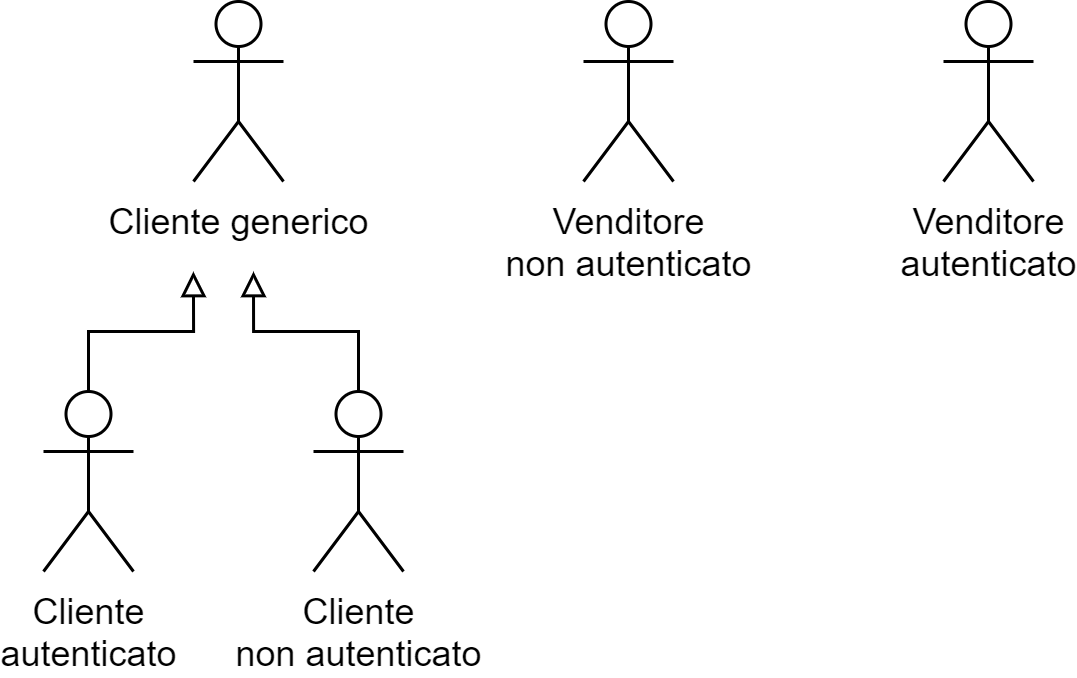
\includegraphics[width=32em]{res/images/UC/attori.png}
    \caption{Diagramma attori} 
\end{figure}
\subsubsection{Attori Principali}
\begin{itemize}
    \item \textbf{Cliente generico:} cliente che naviga la piattaforma e può usarne la maggior parte delle funzionalità come navigazione, ricerca, aggiunta al carrello del prodotto, acquisto. Si differenzia in: 
    \begin{itemize}
        \item \textbf{Cliente autenticato:} cliente che ha superato la fase di login e può accedere alle funzionalità riservate ai clienti autenticati.
        \item \textbf{Cliente non autenticato:} cliente che non ha ancora eseguito il login oppure non è ancora registrato alla piattaforma. 
    \end{itemize}
    \item \textbf{Venditore non autenticato:} venditore che non ha ancora effettuato il login.
    \item \textbf{Venditore autenticato:} venditore che ha effettuato il login con successo. Può accedere a tutta la sezione riservata della piattaforma dove può amministrare tutte le funzionalità (amministrazione prodotti, amministrazione categorie, amministrazione piattaforma).
\end{itemize}
